\documentclass[12pt]{scrartcl}
\usepackage[utf8]{inputenc}
\usepackage[english]{babel}
\usepackage{underscore}
\usepackage[hidelinks]{hyperref}
\hypersetup{linktoc=all}

\usepackage{setspace}
\usepackage{lastpage}
\usepackage{extramarks}
\usepackage{chngpage}
\usepackage{titling}
\usepackage{listings}
\usepackage{float}

\title{KBS Assignment Bayes B}
\author{Lennart Purucker, Thore Krüss}
\date{\today}

\usepackage{graphicx}


\usepackage{makeidx}
\makeindex

\usepackage{fancyhdr}
\pagestyle{fancy}

\fancyhf{}

\rhead{\thetitle}
\lhead{\theauthor}
\rfoot{\thepage~/~\pageref{LastPage}}
\setlength{\headheight}{15pt}

\begin{document}

\maketitle

\tableofcontents

\newpage

\section{Introduction}
\label{sec:intro}
We have used the Framework Netica (Java API Version) from Norsys to build a bayesian network that classifies a case (accumulation of input variables) to a tariff A or B.

We have chosen Netica because it is the best tool to visualize and reuse created networks even though the library structure, documentation and code feels like an artifact.

Java was chosen since it is the best version of the Netica API that fits our own skill set. Organically, other Python libraries were looked at but later discarded due to their lack of required features (like and especially visualization).

The goal has been to build tool that is as dynamic as possible by having all network properties defined by input files or automatically adjusted by the tool itself.

\subsection{Netica Docs}
\begin{itemize}
    \item Netica Homepage: \url{https://www.norsys.com}
    \item Netica Java Manual: \url{https://www.norsys.com/netica-j/docs/NeticaJ_Man.pdf}
    \item \textbf{Notice}: The free version of Netica only supports networks with 15 nodes.
\end{itemize}

\subsection{Documentation Content}
The documentation for this projects consists of 4 sections (including this one) which describe everything notable about this project.
\begin{itemize}
    \item This section will go into the idea and goal of the project (Intro)
    \item The data documentation (\autoref{sec:data_doc}) does contain information about the input data CSV files (Assumptions, content, etc).
    \item The code documentation (\autoref{sec:code_doc}) does note additional information about the code and explain the basics.
    \item Getting started (\autoref{sec:getting_started}) will describe the normal workflow to run this Application on Windows and how to use the Netviewer.
\end{itemize}

\subsection{Folder Structure}
\begin{itemize}
    \item The \texttt{imgs} folder holds a set of images which display older and the newest version of link setup for our network.
    \item The \texttt{src} folder holds the app and code we have created.
    \item The \texttt{NeticaJ_Win} folder holds the Netica Java library
    \item The \texttt{data} folder contains any input data
    \item The \texttt{results} folder contains all output files (also temporary files)
    \item The \texttt{build} folder functions as a simpler pre compiled runnable version of the code.
\end{itemize}

\subsection{Execution Plan}
The following is a list of steps performed by this program. It is also visualized in \autoref{fig:exec_plan}.
\begin{enumerate}
    \item The program extracts all possible nodes and values (possibilities) from a CSV input file.
    \item The program builds nodes with the data from the CSV file.
    \begin{itemize}
        \item The possibilities will be normalized (to string) and sets of numbers will be transformed into ranges (strings). This is done to fit to Neticas input options.
    \end{itemize}
    \item The program will link all nodes accordingly to a CSV file that describes the desired links.
    \item The program wil learn CPTs from the original input data.
    \begin{itemize}
        \item CSV file data will be mapped to normalized possibilities and put into a Netica CaseFile (also saved to the output folder).
    \end{itemize}
    \item The program will classify input test data given by a csv file and displays results of the classification.
    \item The Network will be saved into a .dne file.

    \item The network can be displayed, tested and examined within a Netviewer (based on Netica Netviewer Example class).
    \begin{itemize}
        \item This can be done after the network has been saved by starting the Netviewer.
        \item This could also be done by using the normal Netica app.
    \end{itemize}
\end{enumerate}

\begin{figure}[H]
    \centering
    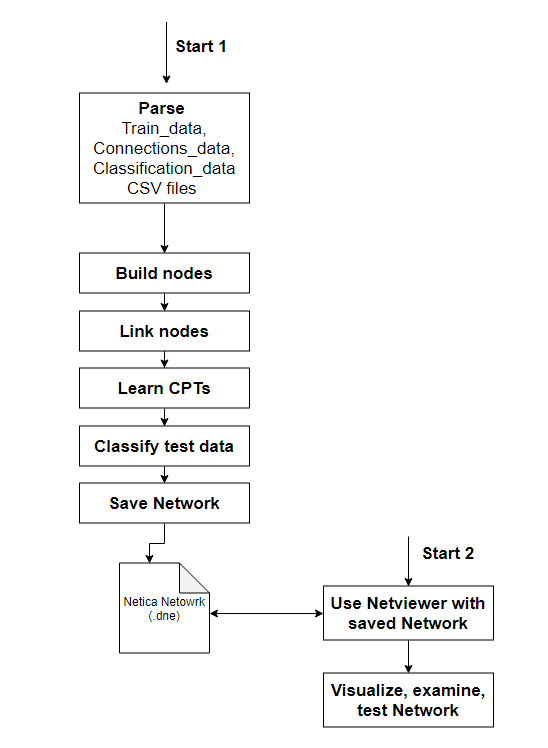
\includegraphics[height=0.8\textheight]{img/workflow.PNG}
    \caption{Execution Plan}
    \label{fig:exec_plan}
\end{figure}

\subsubsection{Further Netica notes}
\begin{itemize}
    \item We decided against using synthetic nodes because we could only use a single additional one if we would have used them (du toe cap of 15 nodes). This would not have been enough for our ideal setup. Additionally the CPT learning for synthetic nodes did not work correctly.
    \item Our CPT learning algorithm is called "counting learning" (see NeticaJ manual). We used this implementation because it was the best fit for our code structure.
    \item The example data is heavily biased (more than 50\%) towards the result "B". This made the CPT learning algorithm creating CPTs which are also statistically "biased" towards "B". This resulted in better classification for "B" and worse for "A" in most cases. We did look into editing, creating or modifying our training data against this bias but stopped after we decided that this was out of scope. We also considered different methods to partition the given dataset into test and training data, such as the K-Folds-Method but discarded them as out of scope and we considered the effect not to be reasonable enough.
    \item We decided to create discrete variables from possible (positive) continuous ones by deducing ranges from all given cases with the help of boxplots. This is now done automatically be the program. Hereby any "n.a." value will be mapped to the lowest range and zero is the lowest possible value even if the boxplot would have been lower.
\end{itemize}



\subsubsection{Learning/Training}
We tested different Network connections with different test/training data. Our current Test Data (\texttt{data/versicherung_a_classify.csv}) will create the final output as in \autoref{lst:test_data}.


\begin{lstlisting}[breaklines, caption={Output of a program execution with given test data},label={lst:test_data}]
3 cases did not have a control result.
15 of 17 cases are correct! Ratio: 88.2353 %
For cases with result B: 11 of 11 cases are correct! Ratio: 100.0 %
For cases with result A: 4 of 6 cases are correct! Ratio: 66.66667 %
64.70589 % of all cases are with the result B
35.294117 % of all cases are with the result A
\end{lstlisting}

This shows the possibilities for all results of all classifications.  Every single classification will also be shown with its input and percentages.
The test dataset also contains empty (falsified) data from the original dataset to test different input possibilities.

\begin{itemize}
    \item In this fashion, several connection setups were created and tested that created certain results when being trained and tested with all given data.
    Three of these connection setups can be found under \\ \texttt{data/connectionSetup}.\\
    Here the ending has to be read like follows: "O" indicates the overall correct ratio, "B" the ratio for correctness of B and "A" for the correctness of A.
    The connection setup with the highest success rate in our tests was the connection setup that we explain in \autoref{sec:node_structure} and created logically before we modified one link after testing.
    This has been used as the standard for now (just \texttt{netConnections.csv}).
    \item The interconnection and relations of nodes and different test data can be examined pretty good in the Netviewer where you can do inference by hand.
\end{itemize}

\subsection{Creating a node structure}
\label{sec:node_structure}
For Netica to provide reasonable results it was necessary to declare dependencies between nodes.
In the first iteration we wanted to use synthesized nodes to group certain categories (the draft can be seen in \autoref{fig:synthesized_nodes}).
Due to limitations in Netica (node limitation and no proper CPT learning) we decided to abolish the idea and only use given nodes.
The newly created concept is shown in \autoref{fig:final_setup} including comments for the connections providing the reasoning behind the decision.
The final network created and with CPTs learned by Netica utilizing the given sample data set is shown in \autoref{fig:netica_final}.

\begin{figure}[H]
    \centering
    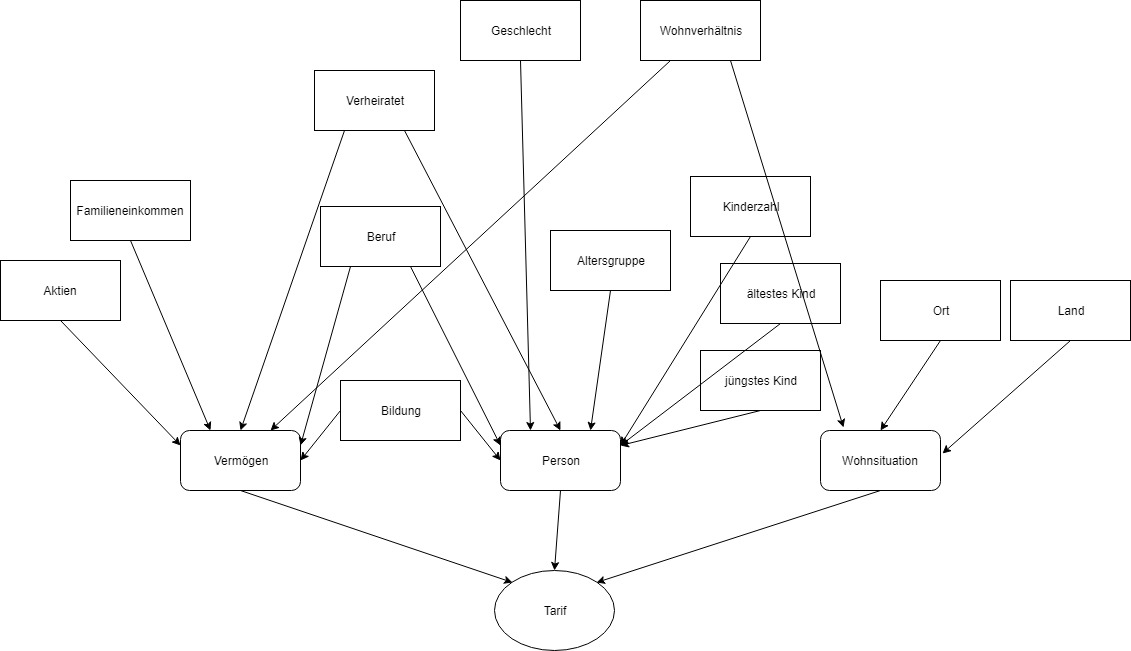
\includegraphics[width=.9\textwidth]{img/connectionsV1.jpg}
    \caption{First draft with synthesized nodes}
    \label{fig:synthesized_nodes}
\end{figure}

\begin{figure}[H]
    \centering
    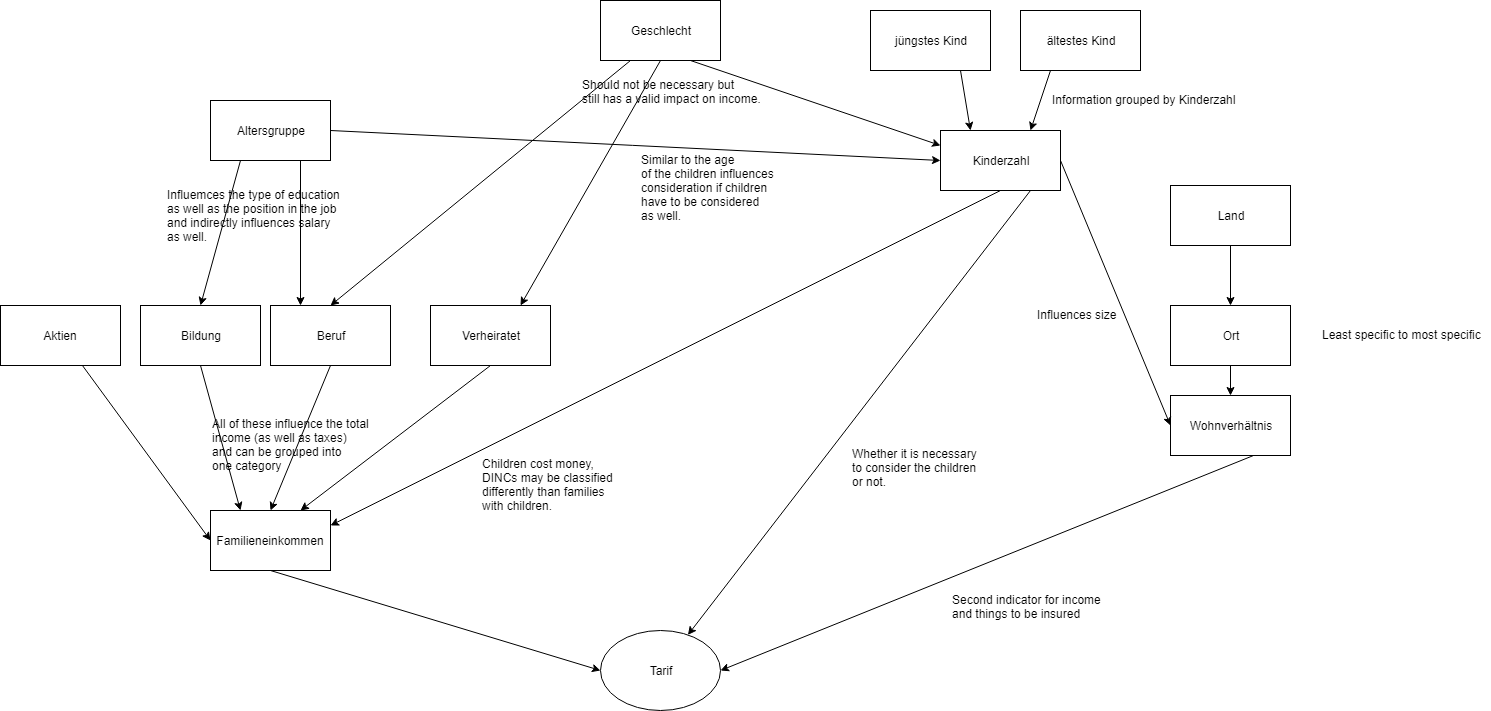
\includegraphics[width=.9\textwidth]{img/connectionsv2.png}
    \caption{Final setup with comments explaining the connections}
    \label{fig:final_setup}
\end{figure}

\begin{figure}[H]
    \centering
    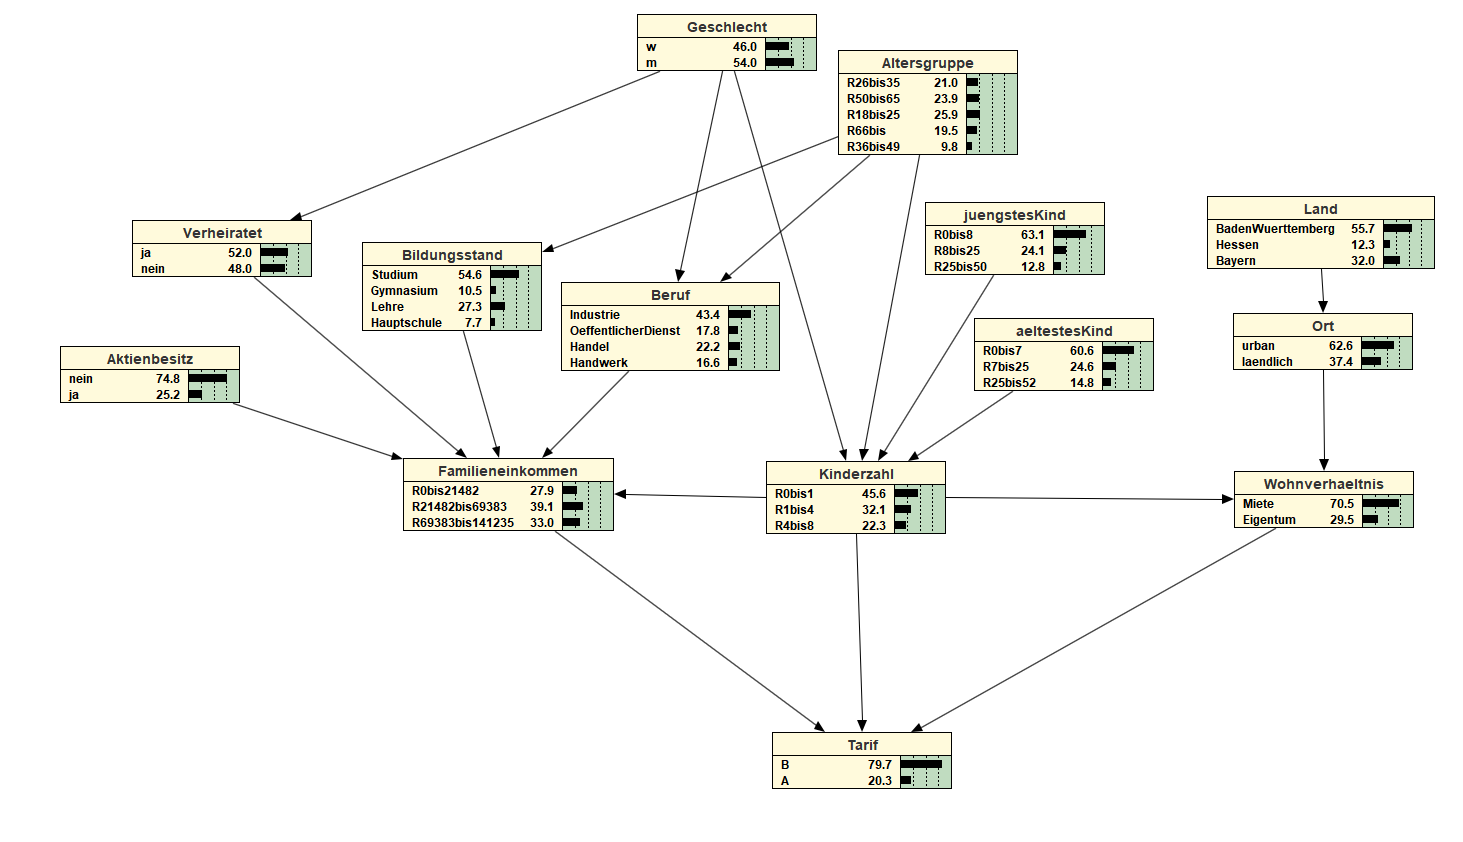
\includegraphics[width=.9\textwidth]{img/currentConnectionSetupWithLearnCPTs.png}
    \caption{Setup learned by Netica with CPTs}
    \label{fig:netica_final}
\end{figure}


\section{Data Structure}
\label{sec:data_doc}
This is the documentation about assumptions and constraints for all input files.

All input files are stored in the \texttt{data/} directory or its sub-directories.

\subsection{Training Data -- CSV file (.csv)}
The training data csv file (in this project \texttt{versicherung_a.csv}) contains information about all possible nodes and values.
This data is used to obtain all nodes and possibilities and building a case file to train the CPTs.

The current example is given under \texttt{data/versicherung_a.csv}

\subsubsection{Assumptions}
\begin{itemize}
    \item First line contains the column headers (nodes of the network)
    \item Last column contains evaluation information (e.g. assigned product A/B).
    \item Only two evaluation results exist (e.g. A and B).
    \item Values are separated by a semicolon.
    \item No usage of quotes but raw strings instead.
    \item "Empty" numeric values are marked with "n.a.", non numeric vales should not be empty.
    \begin{itemize}
        \item They could be empty but this would be not beneficial.
    \end{itemize}
    \item The minimum a numeric value could attain is zero.
    \item No empty lines and each line has "content" (e.g. semicolons) for each node
\end{itemize}


\subsection{Test data -- CSV file (.csv)}
This test data csv file supplies data that is used for the classification test. It is similar to the training data csv file but has further assumptions.

Current example is given under \texttt{data/versicherung_a_classify.csv}

\subsubsection{Assumptions}
\begin{itemize}
    \item First line contains the column headers (nodes of the network).
    \item Last column contains evaluation information (e.g. assigned product A/B).
    \begin{itemize}
        \item This can be empty but if a control value is given, statistics will be created for correct/false classifications.
    \end{itemize}
    \item Only two evaluation results exist (e.g. A and B).
    \item Values are separated by a semicolon.
    \item No usage of quotes but raw strings instead-
    \item "Empty" numeric values are marked with "n.a." and can be empty, non numeric vales can be empty.
    \begin{itemize}
        \item An all empty line will return the default CPT table of the evaluation node as result (e.g. the actual distribution).
        \item Missing values are not used for the classification (as intended) but a result can still be produced.
    \end{itemize}
    \item The minimum a numeric value could attain is zero.
    \item No empty lines and each line has "content" (e.g. semicolons) for each node.
\end{itemize}

\subsection{Network Links -- CSV file (.csv)}
This file describes the links between nodes that shall be implemented for the network. This provides a non hard coded possibility to setup the links between the nodes.

\begin{itemize}
    \item Our default connection Setup is given under\\ \texttt{data/connectionSetup/netConnections.csv}.
    \item Other connection setups are given as well in this directory. The name contains its statistics.
    \item Here the ending has to be read like this: "O" indicates the overall correct classification ratio, "B" the ratio for correctness of B and "A" for the correctness of A.
\end{itemize}

\subsubsection{Assumptions}
\begin{itemize}
    \item First element is the target node for a link, rest of the row are elements that point to this target node (first element of row)
    \item Everything is a string and separated by ";"
    \item Every string uses ASCII characters (e.g no "ö" etc)
    \item Every pointerNode of a target node is unique
    \item no trailing ";"
    \item No empty lines
\end{itemize}


\section{Code}
\label{sec:code_doc}
A lot of in-code documentation exits and should make the code understandable. Here are some "justifications" why we did stuff the way we did it (most of the time the reason is Netica).
Additionally a short overview about all functions will be presented.

All code is stored in the \texttt{src/app/Main.java} file.

\subsection{Justifications}
As Python native developers some of the code structure we had to use because of Java and Netica where not "normal". Therefore we justify them in the following key points.

\begin{itemize}
    \item To make our Netica code run we had to build a one-file app. Thus all classes had to be put into one file. This creates a very unclean class monolith but was our only working option for Netica.
    \item A lot of our code is surrounded by try-catch statements. This has to be done because every part of Netica code throws exceptions.
    \item When creating a node, you have to assign it to a new node object even though just calling the constructor would do just fine because it adds it to the network.
    \item For the possibilities of nodes (e.g. node states) the set of all values has to be either string or integer. We wanted strings and thus mapped all integer values to ranges that are string objects.
    \item To have a common structure: If the possibility is a number $\rightarrow$ $N$ indicates pure numbers, $R$ indicates a range.
    We chose this convention to be able to utilize strings as inputs and not keep track of conversion tables to numbers. This makes the network more readable for netviewer and our own classification.
    \item Similar we had to change input values because Netica does not use a list object or something like that but a raw string with separators like "." or ",". Thus these chars had to be replaced as well.
    \item For some reason "-" is an invalid character in netica. Thus it was replaced by "bis".
    \item Ranges exclude the upper limit and include the lower limit.
\end{itemize}


\subsection{Class Overview}
\begin{itemize}
    \item \texttt{Main}: The static entry point and main execution part of the code
    \item \texttt{NeticaNetBuilder}: A class which builds the a Netica Net for given input data (nodes, links, CPTs).
    \item \texttt{CSVUtils}: CSV Reader/Parser Class.
    \item \texttt{Utils}: Contains several non class-specific utility functions (which could be reused somewhere else).
    \item \texttt{NeticaUtils}: Utils code for Netica (like Net "constructor" and "deconstructor").
    \item \texttt{NeticaClassifyData}: Class to classify given input data for a given netica net.
\end{itemize}

%![Class connections image](./classConnections.PNG "Project structure")
\begin{figure}[H]
    \centering
    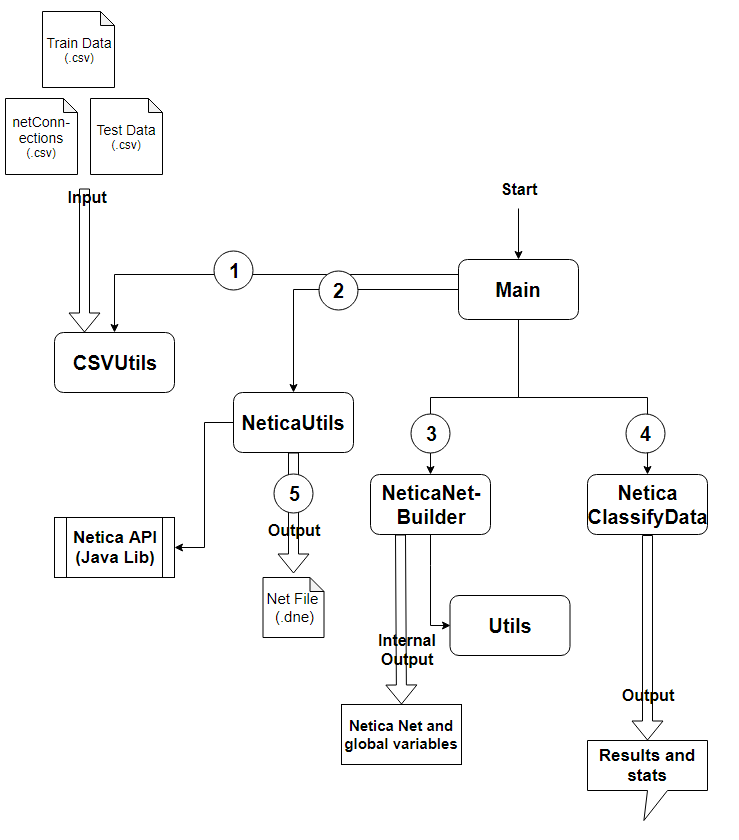
\includegraphics[width=.9\textwidth]{img/classConnections.PNG}
    \caption{Class structure}
    \label{fig:class_structure}
\end{figure}



\section{Executing the implementation}
\label{sec:getting_started}
This section shall provide a short overview of how to get the program started within this project.

\begin{itemize}
    \item The application builds the network, does classification for a set of data and saves the network.
    \item The Netviewer allows you to view, examined and play with the network in an application format.
    \item This is a default Netica app and could also be replaced by the actual Netica App. It has similar features.
    \item So far a simpler executable version was not possible due to Netica not being a library.
\end{itemize}

\subsection{Build (pre-compiled) version}
Even so this is a pre-compiled version, a JDK is still needed.
Additionally, Netica code has to be executed with certain Netica path variables which will be temporally set for the execution by the ".bat" files.
This made it impossible to create a "normal" JAR executable or provide a ".exe" bundled "JAR" Version.

Simply navigate to the \texttt{build} folder and execute the \texttt{.bat"} files. Both can be executed from the Windows file explorer with a double click or from the CLI.

For the usage of Netviewer see \autoref{sec:netviewer}

\subsubsection{BayesInsurance}
Double click \texttt{run_bayesInsurance.bat} or do \texttt{.\textbackslash run_bayesInsurance.bat} in the CLI using different csv files/path or names for files.

\subsubsection{Troubleshooting}
\begin{itemize}
    \item Make sure the path is set correctly and calling just \texttt{java} in the command line prompts a default manual response and not an command not found error.
    \item Sometimes Netica code only runs on 32 bit JDKs thus 64 bit Version could be a problem. Workaround:
    \begin{enumerate}
        \item Download and install 32 bit JDK.
        \item Setup your Java path correctly to include a 32 bit Version of the JDK (Make sure its the x86 path (for 32 bit)\footnote{See \url{https://stackoverflow.com/a/8518438} for help}.
    \end{enumerate}
\end{itemize}

\subsection{Run the code (on Windows)}

\subsubsection{Setup for Windows}
\begin{enumerate}
    \item Download/Clone/Copy this project (with all its files)
    \item Setup your Java path correctly to include a 32 bit Version of the JDK
    \begin{itemize}
        \item See for help: \url{https://stackoverflow.com/a/8518438}
        \item Make sure its the x86 path (for 32 bit).
        \item This has to be done for the Netica Java version which needs this 32 bit JDK.
    \end{itemize}
\end{enumerate}

\subsubsection{Start the Application}
\begin{enumerate}
    \item Go to the \texttt{/src} folder
    \item Execute \texttt{compile_and_run_app.bat} in CMD or Powershell.
    \begin{itemize}
        \item This will compile the Java code with Netica for your system and run it afterwards.
    \end{itemize}
\end{enumerate}

\paragraph{Using different CSV files} can be achieved editing the \texttt{src/compile_and_run_app.bat} and setting the new path in the last line after "Main".

\subsection{Netviewer}
\label{sec:netviewer}
\begin{enumerate}
    \item Go to \texttt{src/netviewer}
    \item Run \texttt{compile_and_run_netviewer.bat}
\end{enumerate}

\subsubsection{NetViewer Workaround}
Sadly the Netviewer from netica is not working properly. Thus the following has to be done to see the net correctly.

\textbf{Problem}: Default saved netica network wont be displayed in the center of the app

\begin{enumerate}
    \item Start the Netviewer (Use it in full screen)
    \item Click on "File" $\rightarrow$ "Open" and select the correct net file (".dne") and click open again
    \item In the row "Node Styles" select "Circle"
    \item A circle object should appear in the left top corner
    \item Drag and drop one of the circles to the middle/bottom right of the screen
    \item In the row "Node styles" select "Auto Select"
    \item Now you can see the Network. Move the boxes (drag and drop) accordingly to build yourself a better view of the network.
\end{enumerate}


Additionally the Netviewer can work as a GUI to enter cases etc.


\end{document}
